\documentclass[english,serif,mathserif,xcolor=pdftex,dvipsnames,table]{beamer}
\usetheme{gc3}

\usepackage[T1]{fontenc}
\usepackage[utf8]{inputenc}
\usepackage{babel}

\usepackage{gc3}

\title[Workflows]{%
  Introduction to workflows with GC3Pie
}
\author[R. Murri, S3IT UZH]{%
  Riccardo Murri \texttt{<riccardo.murri@uzh.ch>}
  \\[1ex]
  \emph{S3IT: Services and Support for Science IT}
  \\[1ex]
  University of Zurich
}
\date{January~23--27, 2017}


\begin{document}

% title frame
\maketitle


% \begin{frame}
%   \frametitle{The GC3Pie approach to workflows, I}

%   \begin{center}
%     Workflows are Python code.
%   \end{center}
% \end{frame}


% \begin{frame}
%   \frametitle{The GC3Pie approach to workflows, II}

%   Thus, in order to run a workflow, you write a Python script using
%   GC3Pie to orchestrate the running of applications.

% \end{frame}


\begin{frame}

  So far we've seen how to write scripts that control many instances of
  a single application.

  \+
  Now it's time to introduce the GC3Pie classes that allow
  orchestrating the execution of jobs of several different types. (For
  instance, specify that certain applications should be executed in a
  sequence.)

  \+
  Let's start with a colorful example.
\end{frame}


\begin{frame}
  \frametitle{Warholize!}

  \begin{tabular}[c]{ccc}
    \includegraphics[width=0.4\textwidth]{fig/butterfly.jpg}
    &
    {\includegraphics[width=0.1\linewidth,totalheight=0.25\textheight]{fig/arrow.pdf}}
    &
    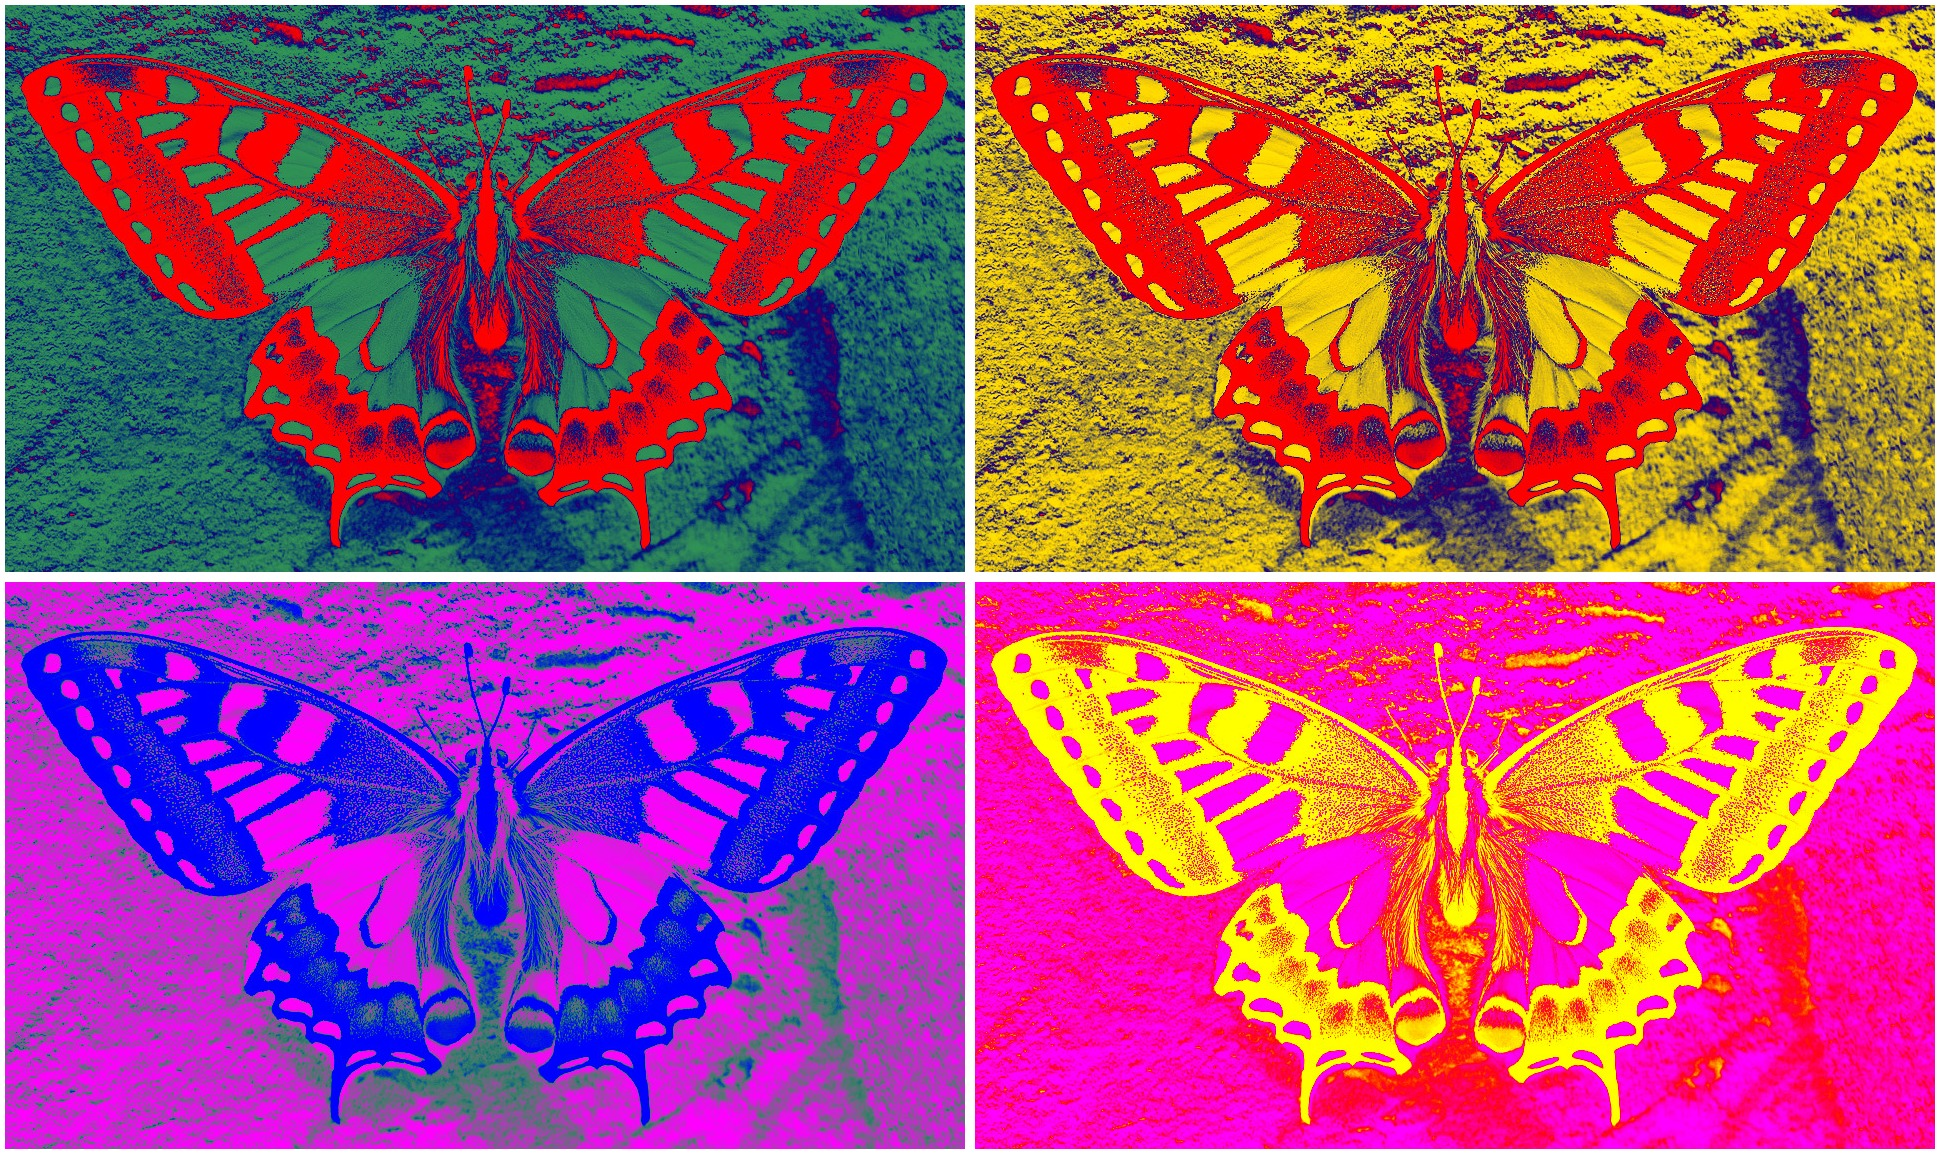
\includegraphics[width=0.4\textwidth]{fig/warholized-butterfly.jpg}
  \end{tabular}
\end{frame}


\begin{frame}[fragile]
  How do we ``warholize'' an arbitrary image?

  \+
  \begin{enumerate}
  \item Convert the original image to grayscale.
  \item Colorize the grayscale image using three different colors for each tile.
  \item Arrange all the colorized images into an $N\times N$ frame.
  \end{enumerate}

  \+
  \begin{references}
    \url{http://gc3pie.readthedocs.io/en/master/programmers/tutorials/index.html#warholize-tutorial}
  \end{references}
\end{frame}


\begin{frame}
  \frametitle{The GC3Pie approach to workflows, II}

  The basic unit of work in a GC3Pie workflow is called a \texttt{Task}.

  \+
  The \texttt{Application} class that you already know is a kind of
  \texttt{Task} (indeed, it's a derived class).

  \+
  From now on, we'll speak of \texttt{Task}s rather than
  applications.  Examples of \texttt{Task} instances that are not
  applications will arrive shortly.
\end{frame}


\begin{frame}
  \frametitle{Running tasks in sequence}

  To run tasks in an ordered sequence, one after the other, GC3Pie
  provides a \texttt{SequentialTaskCollection} class.

  \+
  It is created with a list of tasks, and runs all of them in the
  order given.  The sequence is dynamic, in that you can add new tasks
  on the fly, re-run existing ones, or remove future tasks.

  \+
  A \texttt{SequentialTaskCollection} is itself a task.
\end{frame}


\begin{frame}
  \frametitle{Running tasks in parallel}

  To run tasks in parallel (i.e., they have no inter-dependency),
  GC3Pie provides a \texttt{ParallelTaskCollection} class.

  \+
  It is created with a (Python) list of tasks, and runs all of them
  in parallel (compatibly with the computational resource limits).

  \+
  A \texttt{ParallelTaskCollection} is itself a task.

\end{frame}


\begin{frame}
  \frametitle{Putting it all together}
  So tasks can be:
  \begin{itemize}
  \item \texttt{Application} instances,
  \item \texttt{SequentialTaskCollection}s,
  \item \texttt{ParallelTaskCollection}s.
  \end{itemize}

  \+
  So you can nest them, and create parallelly-running sequences, or
  sequences of ``task explosions'' (many tasks in parallel), or any
  combination of this.
\end{frame}


\begin{frame}
  \frametitle{The Warholize workflow, I}

  {\color{gray}\itshape 1.}
  Convert the original image to grayscale.

  \+
  \includegraphics[height=0.60\textheight]{fig/warholize-wkf1}
\end{frame}


\begin{frame}
  \frametitle{The Warholize workflow, II}

  {\color{gray}\itshape 2.}
  Colorize the grayscale image using three different colors for each tile.

  \+
  \includegraphics[height=0.60\textheight]{fig/warholize-wkf2}
\end{frame}


\begin{frame}
  \frametitle{The Warholize workflow, III}

  {\color{gray}\itshape 3.}
  Arrange all the colorized images into an $N\times N$ frame.

  \+
  \includegraphics[height=0.60\textheight]{fig/warholize-wkf3}
\end{frame}


\begin{frame}
  \frametitle{The Warholize workflow, IV}

  Step~\textit{2.} actually entails two sub-steps:
  \begin{enumerate}[a)]
  \item mapping greyscale levels to random colors,
  \item applying this mapping to produce new images
  \end{enumerate}

  \+
  \includegraphics[height=0.60\textheight]{fig/warholize-wkf2a}
\end{frame}


\begin{frame}
  \frametitle{The Warholize workflow, V}

  So, Step~\textit{2.} is a \texttt{SequentialTaskCollection}-type task.
  Let's call this two-pass sequence \texttt{TricolorizeImage}.

  \+
  \includegraphics[height=0.60\textheight]{fig/warholize-TricolorizeImage}
\end{frame}


\begin{frame}
  \frametitle{The Warholize workflow, VI}

  All the \texttt{TricolorizeImage} instances run in parallel. Collect
  them into a \texttt{ParallelTaskCollection}-type task, called
  \texttt{TricolorizeMultipleImages}.

  \+
  \includegraphics[height=0.60\textheight]{fig/warholize-TricolorizeMultipleImages}
\end{frame}

\begin{frame}
  \frametitle{The Warholize workflow, VII}

  Now we are left with a three-step sequence: greyscale,
  \texttt{TricolorizeMultipleImages}, montage.  This can be defined
  again as a \texttt{SequentialTaskCollection}-type task, the
  \texttt{WarholizeWorkflow}.

  \+
  \includegraphics[height=0.60\textheight]{fig/warholize-WarholizeWorkflow}
\end{frame}


\end{document}

%%% Local Variables:
%%% mode: latex
%%% TeX-master: t
%%% End:
